\documentclass{beamer}
\usepackage[citestyle=authoryear, style=authoryear, backend=biber, uniquename=init, giveninits=true]{biblatex}
\usepackage{lmodern}
\usepackage{amsmath,amssymb}
\usepackage{mathtools}
\usepackage[version=3]{mhchem} % Formula subscripts using \ce{}, e.g., \ce{H2SO4}
\usepackage{siunitx}
\usepackage[utf8]{inputenc}
\usepackage{caption}
\captionsetup[figure]{labelformat=empty,justification=centering}
% https://tex.stackexchange.com/a/155611/56227
\usepackage{textcomp}
\usepackage{todonotes}
% footnote per page https://tex.stackexchange.com/a/1088/56227
\usepackage{perpage}
% speaker notes
\usepackage{pgfpages}
\usepackage{hyperref}

% siunitx setup
\sisetup{group-separator={,},
	detect-all,
	binary-units,
	list-units = single,
	range-units = single,
	range-phrase = --,
	per-mode = symbol-or-fraction,
	separate-uncertainty = true,
	multi-part-units = single,
	list-final-separator = {, and }
	%    scientific-notation = fixed
}

\newcommand{\textapprox}{\raisebox{0.5ex}{\texttildelow}}

% \setbeameroption{hide notes} % only slides
% \setbeameroption{show only notes} % only notes
\setbeameroption{show notes on second screen=right} % both

\graphicspath{{./Figures/}}

% clear title and doi from citations
% from https://tex.stackexchange.com/q/165481/56227
\AtEveryCitekey{\clearfield{doi}\clearfield{title}}

% use dash for range phrase by default, and one unit
\sisetup{range-phrase=--, range-units = single}

% turn off nav bar
\beamertemplatenavigationsymbolsempty

% footnote per page https://tex.stackexchange.com/a/1088/56227
\MakePerPage{footnote}

% symbols for footnotes
\renewcommand{\thefootnote}{\fnsymbol{footnote}}

%smaller footnotes, adapted from http://tex.stackexchange.com/a/146021
\setbeamerfont{footnote}{size=\fontsize{6pt}{0pt}}
\setbeamerfont{mpfootnote}{size=\fontsize{6pt}{0pt}}

% numeric footnote symbols
\def\thefootnote{\arabic{footnote}}
\def\thempfootnote{\arabic{mpfootnote}}

% set themes
\usetheme{Frankfurt}
\usecolortheme{seahorse}
\usefonttheme{serif}

% adjust footnote width
%\newlength{\tmpwidth}
%\setlength{\tmpwidth}{0.65\paperwidth}
%\addtobeamertemplate{footnote}{\hsize\tmpwidth}{}

%footnote spacing avoids navigation / margins, adapted from http://tex.stackexchange.com/a/44231
%\addtobeamertemplate{footnote}{\vspace{-6pt}\advance\hsize-0.5cm}{\vspace{6pt}}
%\makeatletter
% Alternative A: footnote rule
%\renewcommand*{\footnoterule}{\kern -3pt \hrule \@width 2in \kern 8.6pt}
% Alternative B: no footnote rule
% \renewcommand*{\footnoterule}{\kern 6pt}
%\makeatother

%make frame for each section
\AtBeginSection[]{
  \begin{frame}
  \vfill
  \centering
  \begin{beamercolorbox}[sep=8pt,center,shadow=true,rounded=true]{title}
    \usebeamerfont{title}\insertsectionhead\par%
  \end{beamercolorbox}
  \vfill
  \end{frame}
}

%auto incrementing titles from http://tex.stackexchange.com/a/231533
\newcounter{expensive}
\newcommand\ExpTitle{%
  \frametitle{\refstepcounter{expensive}{Chemical kinetic integration is \textbf{expensive}~--}~\theexpensive}}
\resetcounteronoverlays{expensive}

% define background template env
\newenvironment{background}{%
\usebackgroundtemplate{%
\rule{0pt}{\paperheight}%
\hspace*{\paperwidth}%
\makebox[0pt][r]{
\includegraphics[width=35mm]{logo}}%
}}{}

% space between paragraphs beamer
% https://tex.stackexchange.com/a/22644/56227
\def\parend/{\\~\\}

\bibliography{presentation.bib}

%opening
\title{Accelerating reacting flow simulations via vectorized chemical kinetic integration}
\author{Nick Curtis}
\institute{University of Connecticut}
\date{\today}

\begin{document}

\begin{background}
\maketitle
\end{background}

\begin{background}
\section{Introduction}
\end{background}

\begin{frame}
\frametitle{Improving combustion technology}
The push to design new clean, efficient combustion technologies has driven both:
\begin{itemize}
 \item the development of combustion devices operating in new regimes such as low-temperature combustion as well as,
 \item the creation of large detailed chemical kinetic models for a wide range of fuel classes from bioalcohols~\footfullcite{SARATHY2009852} to gasoline surrogates\footfullcite{SARATHY201867}.
\end{itemize}
These next generation combustion devices are often controlled by chemical processes, rather than current methods which rely on direct physical processes.
\begin{itemize}
 \item reacting-flow simulations can aid in the design process, however the use of \textbf{realistic chemical modeling is critical to obtain predictive results}.
\end{itemize}
\end{frame}

\begin{frame}
 \frametitle{Challenges using realistic chemistry in reacting-flow simulations}
 \textbf{Model size:} Chemical kinetic models for transportation and energy relevant fuels may consist of hundreds to thousands of chemical species, with potentially tens of thousands of reactions (e.g., gasoline \footfullcite{Mehl:2011cn} and jet fuel\footfullcite{Naik2011434})\parend/
 \textbf{Range of scales:} A typical reacting-flow simulation encompasses a wide range of physical and temporal scales, e.g., the flow-through time of a combustion chamber is typically on the order of seconds to milliseconds, while chemical timescales may be just picoseconds in duration\footfullcite{Lu:2009gh} due to the presence of highly reactive radicals and associated short chemical timescales.\parend/
\end{frame}

\begin{frame}
 \frametitle{Numerical stiffness}
 The large range of time-scales present in these chemical kinetic models---known as numerical stiffness---has traditionally been handled by use of implicit integration techniques, which require repeated evaluation and factorization of the chemical kinetic Jacobian.
 \begin{itemize}
  \item Naive implementations of these operations scale \textbf{quadratically} and \textbf{cubically} with the number of species in a model, respectively\footfullcite{Lu:2009gh}.
 \end{itemize}
 Using even modestly sized chemical kinetic models with such a solver can incur severe computation cost (e.g.,~\footfullcite{Moiz2016123}) for realistic reacting-flow simulations.
\end{frame}


\begin{frame}
 \frametitle{Reducing the cost of chemical kinetics}
  A host of techniques have been developed to reduce the cost of chemical kinetic calculations while maintaining fidelity~\footfullcite{turanyi2016analysis}, e.g.:
  \begin{itemize}
   \item removal of unimportant species and reactions,
   \item lumping of species with similar thermochemical properties, and
   \item time-scale methods that reduce numerical stiffness
  \end{itemize}
  Today we will focus on two such (complementary) techniques, analytical Jacobian evaluation and vectorized chemical kinetic integration.
\end{frame}

\begin{background}
\section{Analytical jacobian evaluation}
\end{background}

\begin{frame}
\frametitle{Why use an analytical jacobian?}
\textbf{Accuracy:} the exact chemical kinetic Jacobian evaluation is required for some computational diagnostic methods (e.g., CSP, or CEMA) in addition to non Newton--Krylov based implicit integration techniques\footfullcite{HANSEN2018257} (e.g., a linearly-implicit Rosenbrock methods).\parend/
\textbf{Efficiency:} analytical jacobian evaluation drops the cost from a quadratic dependence on the number of species (for a finite-difference approach) to a linear dependence on the number of reactions in a chemical model\footfullcite{Lu:2009gh}.\parend/
\textbf{Sparsity:} a carefully chosen system of equations can greatly increase the sparsity of the Jacobian~\footfullcite{Schwer2002270}, allowing for fast, sparse linear-algebra and matrix factorization techniques to be used.
\end{frame}

\begin{frame}
 \frametitle{\texttt{pyJac} - an analytical jacobian generator}
 \begin{columns}[c]
  \begin{column}{0.6\textwidth}
  \begin{minipage}[c]{\columnwidth}
    \texttt{pyJac}\footfullcite{Niemeyer:2016aa} is an open-source, validated, chemical kinetic source-rate and analytical Jacobian code-generation platform with thousands of downloads, and has been used in applications such as:
    \begin{itemize}
     \item LES studies of duel-fuel spray combustion (right),
     \item validation\slash performance testing for a DNS code for heterogeneous processors~\footfullcite{HERNANDEZPEREZ201873},
     \item discussion of proper selection of chemical kinetic state variables~\footfullcite{HANSEN2018257}
    \end{itemize}
    \vfill
  \end{minipage}
  \end{column}
  \begin{column}{0.4\textwidth}
    \begin{center}
     \begin{figure}
      \centering
      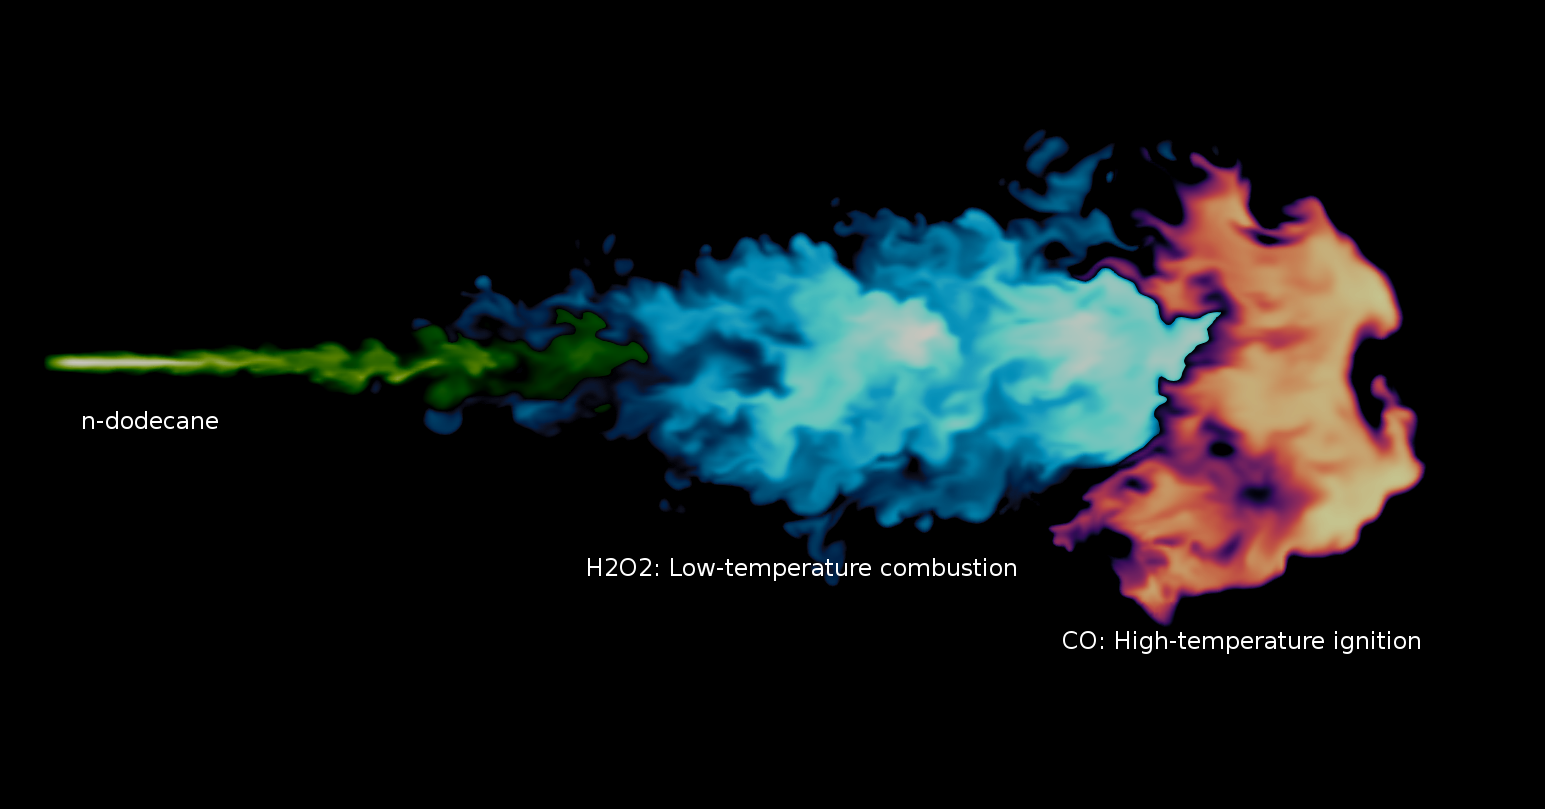
\includegraphics[width=\columnwidth]{spray.png}
      \caption{OpenFOAM LES ECN-Spray A simulation using \texttt{pyJac}}
     \end{figure}
    \end{center}
  \end{column}
 \end{columns}
 \note[item]{The Spray-A simulation is from an upcoming manuscript from Aalto University}
\end{frame}

\begin{frame}
 \frametitle{\texttt{pyJac-V2} - a \textit{better} analytical jacobian generator}
 The initial version of \texttt{pyJac} was capable of vectorized-GPU and multithreaded-CPU operation, \textit{however}:
 \begin{itemize}
  \item no vectorized execution on the CPU (or other accelerators)
  \item the selection of state variables in \texttt{pyJac-V1} meant that the resulting jacobian was almost completely dense
 \end{itemize}
 \textrightarrow Enter\footfullcite{CURTIS2018186} \texttt{pyJac-V2}
\end{frame}

\begin{frame}
\frametitle{Increased jacobian sparsity}
A change of variables lead to a significant increase in Jacobian sparsity (with options available to further increase sparsity at the expense of strict correctness):
\note[item]{the dense lines across the jacobian are due to the presence of the last species in reactions or as a third-body species}
\begin{figure}
 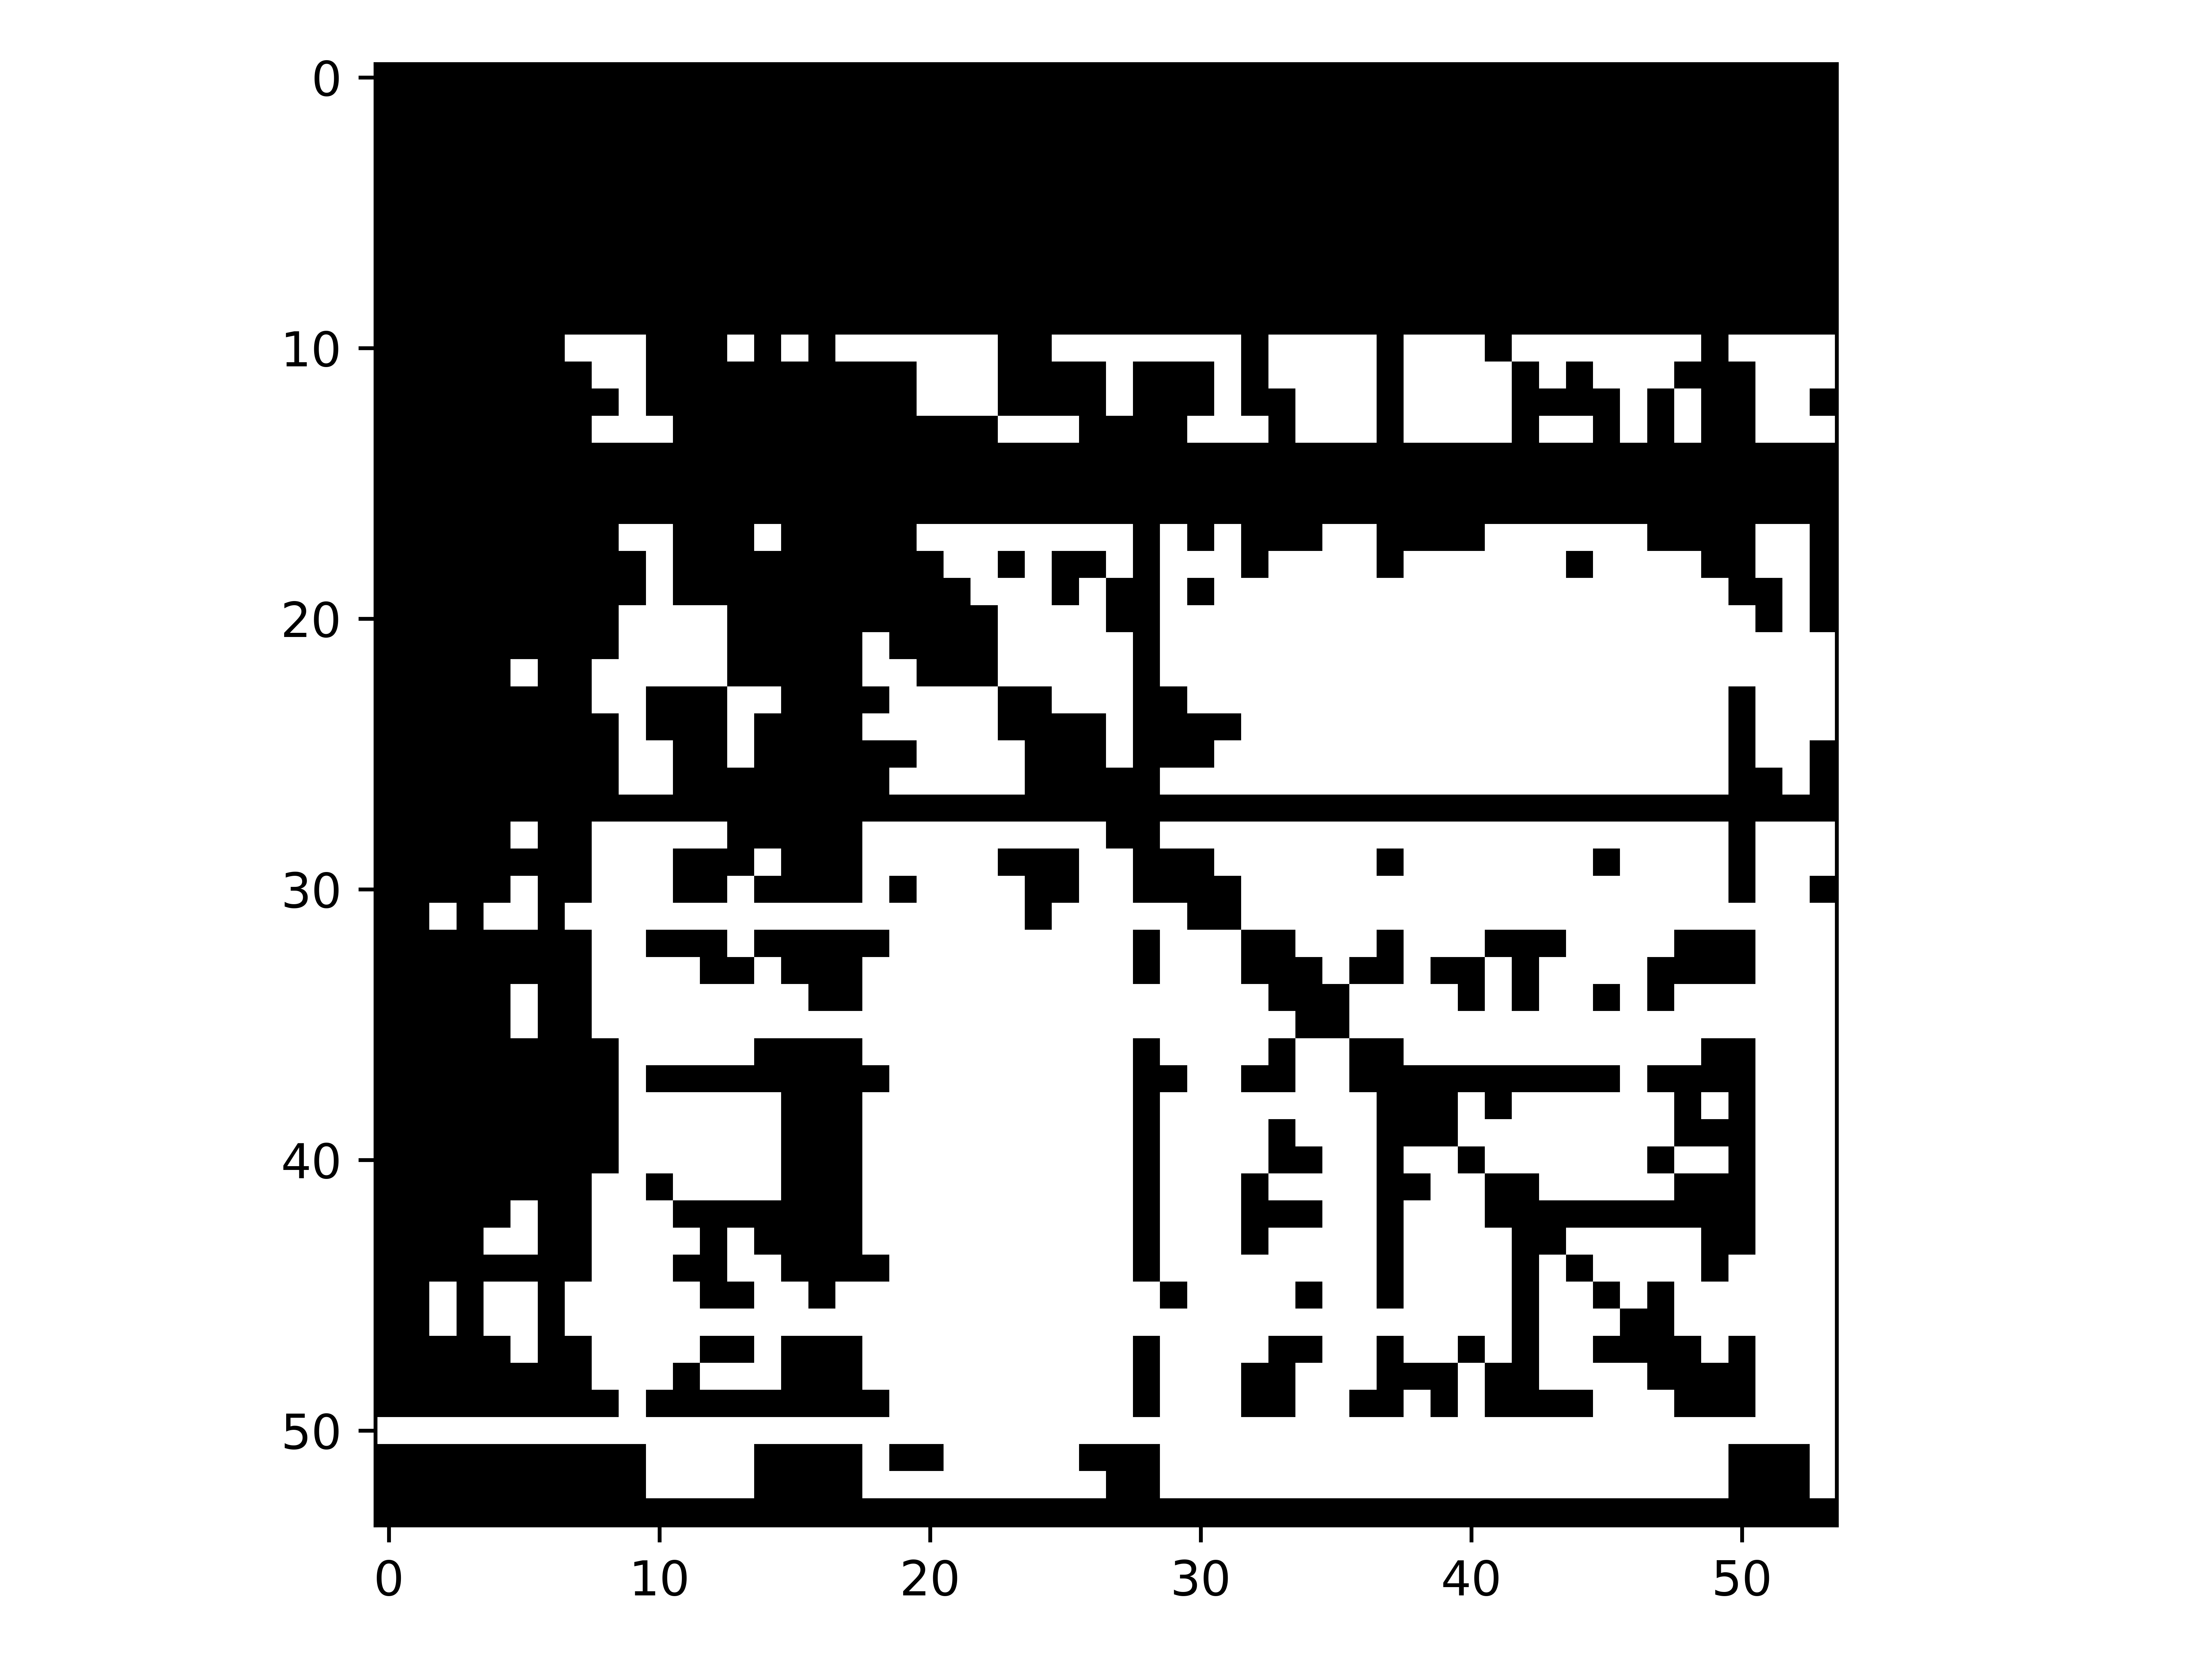
\includegraphics[height=0.5\textheight]{ch4_sparsity_exact.png}
 \caption{Representation of sparsity of GRI-Mech 3.0 chemical kinetic model, a black square indicates a non-zero jacobian entry.}
\end{figure}
\end{frame}

\begin{frame}
\frametitle{Vectorized evaluation on the CPU}
\begin{columns}
 \begin{column}{0.5\textwidth}
  The new version of \texttt{pyJac} utilizes the OpenCL programming language to achieve vectorization on the CPU, GPU and other accelerators.
  \begin{itemize}
   \item achievable CPU-speedup depends on vector-width of the device (\SI{4}{$\times$} here\note[item]{up-to \SI{8}{$\times$} on newest processors}).
  \end{itemize}
  The vectorized CPU code was \SIrange{3.03}{4.23}{$\times$} and \SIrange{6.63}{9.44}{$\times$} faster than purely parallel code (on the same processor) for dense and sparse jacobian evaluation, respectively.
 \end{column}
 \begin{column}{0.5\textwidth}
  \begin{figure}
  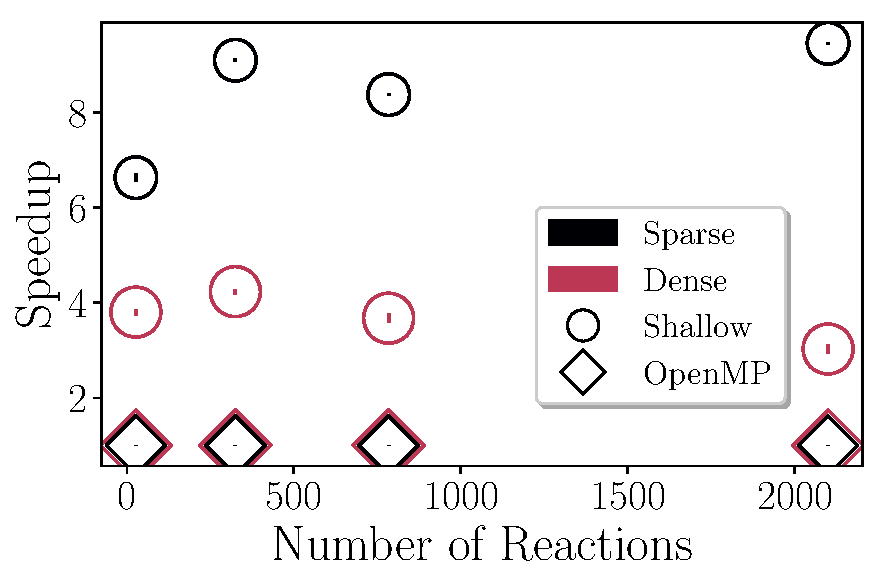
\includegraphics[width=\textwidth]{sparse_vs_dense_speedup.pdf}
  \caption{Speedup achieved by CPU-vectorization of \texttt{pyJac-V2}'s sparse and dense jacobian for several chemical models.}
  \end{figure}
 \end{column}
\end{columns}
\end{frame}


\begin{background}
 \section{Vectorized ODE integration}
\end{background}

\begin{frame}
 \frametitle{Operator splitting and vectorization}
 Many reacting-flow codes utilize operator-splitting techniques (e.g.,~\footfullcite{Knio:1999}$^{,}$~\footfullcite{Ren:2008}) to decouple a large system of partial differential equations, such that different physical processes may be solved independently.
 \begin{itemize}
  \item This results in independent initial value problem (IVPs) of chemical kinetic ODEs at each computational cell in the simulation\textrightarrow~embarrassingly-parallel problem.
 \end{itemize}
\end{frame}

\begin{frame}
 \frametitle{GPU-based chemical kinetic integration}
 Previous works demonstrated the value of GPU-based chemical kinetic integration for non-stiff to moderately-stiff chemistry (e.g.\footfullcite{2014NiemeyerGPU}$^,$\footfullcite{Shi:2012aa}), but efficient GPU-integration of highly-stiff chemistry remained difficult due to issues with thread-divergence\footfullcite{Stone:2013aa}:
 \begin{itemize}
  \item \textit{thread-divergence}: a critical performance concern on GPUs; occurs when different threads must execute different instructions (e.g., branches of an if\slash then statement).
 \end{itemize}
 Newton--Krylov based implicit integration methods tend to be more susceptible to thread-divergence concerns due to the presence of an iteration loop inside of each ODE integration time-step.
\end{frame}

\begin{frame}
 \frametitle{Stiff GPU chemistry integration algorithms}
 Several integration algorithms were tested to determine suitability for GPU-based integration:
 \begin{itemize}
  \item Exponential Rosenbrock methods -- these linearly-implicit techniques do not require Newton iteration inside the integration step\footnote{Ideally, alleviating thread-divergence concerns}, but instead rely on Krylov subspace approximations to the matrix exponential.
  \item Implicit Runge--Kutta method -- a Newton--Krylov method similar to traditionally used methods, but of \textit{fixed} rather than variable-order (as in CVODEs).
  \begin{itemize}
   \item[\textrightarrow] This both simplifies implementation and removes another source of thread-divergence (varying integration order between IVPs)
  \end{itemize}
 \end{itemize}
\end{frame}

\begin{frame}
 \frametitle{Stiff GPU chemistry integration algorithms}
 The developed open-source integration algorithms~\footfullcite{curtis2017investigation} were paired with an analytical Jacobian~\footfullcite{Niemeyer:2016aa}, and tested on chemical models of varying size, and levels of numerical stiffness, finding:%
 \vskip-1.5em
 \begin{columns}[t]
  \begin{column}{0.6\textwidth}
    \begin{itemize}
      \item Speedups for GPU-based implicit Runge--Kutta method, decreased with larger model sizes and global integration time-step size.\note[item]{i.e, with increasing stiffness, 12--38 cores for smaller timestep, 3--15 for larger}
      \item High levels of thread-divergence in the exponential integrators.\note[item]{due to varying integrator step-size and Krylov subspace dimension}
      \item \SIrange{7}{241}{$\times$} speedup on GPU for analytical jacobian versus a finite-difference approach.\note[item]{\SIrange{1.39}{2.69}{$\times$} on CPU}
    \end{itemize}
  \end{column}
  \begin{column}{0.4\textwidth}
   \begin{figure}
    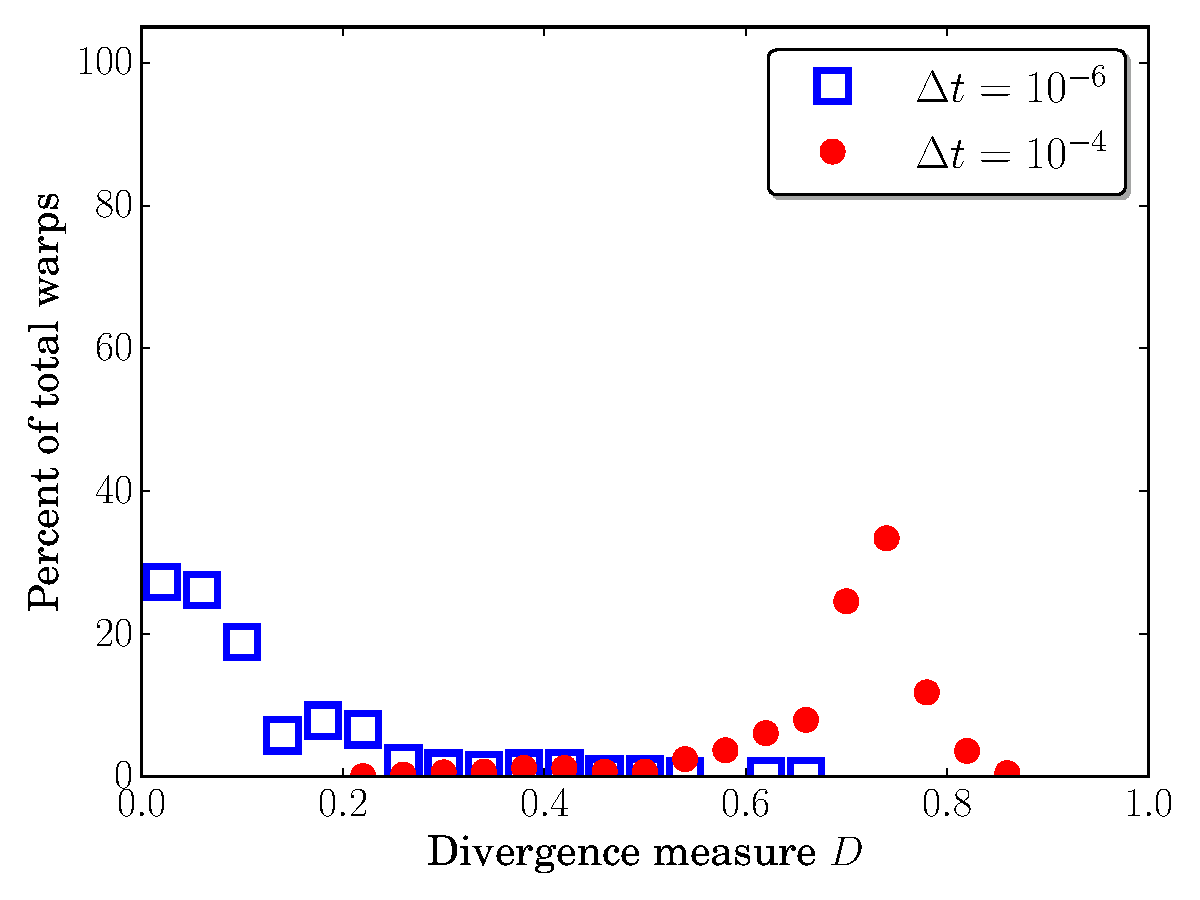
\includegraphics[width=\textwidth]{CH4_exprb43_div}
    \caption{Thread-divergence in the exponential Rosenbrock algorithm for GRI-Mech 3.0.}
   \end{figure}
  \end{column}
 \end{columns}
 \note[item]{So we still have issues with thread-divergence in GPU-solvers\textrightarrow CPU}
\end{frame}

\begin{background}
 \section{Vectorized reacting-flow simulations}
\end{background}

\begin{frame}
 \frametitle{Volvo bluff-body flame}
 To demonstration computational efficiency and accuracy of the algorithms and codes developed thus far, they will be applied to a bluff-body stabilized, turbulent reacting-flame simulation.
 \vskip-1.65em
 \begin{columns}[t]
  \begin{column}{0.6\textwidth}
   \begin{itemize}
    \item OpenFOAM CFD code used to run large eddy simulation
    \item Selected case is well characterized with experimental velocity and temperature measurements available\footnotemark[1]
    \item $U_{\text{in}} = $ \SI{16.6}{\meter/\s}, air at \SI{1}{\bar}, \SI{288}{\kelvin}
    \item \num{2.37e6} mesh nodes (see right), based on recommendations from previous studies\footnotemark[2]$^\text{,}$\footnotemark[3]
   \end{itemize}
  \end{column}
  \begin{column}{0.4\textwidth}
  \begin{figure}
   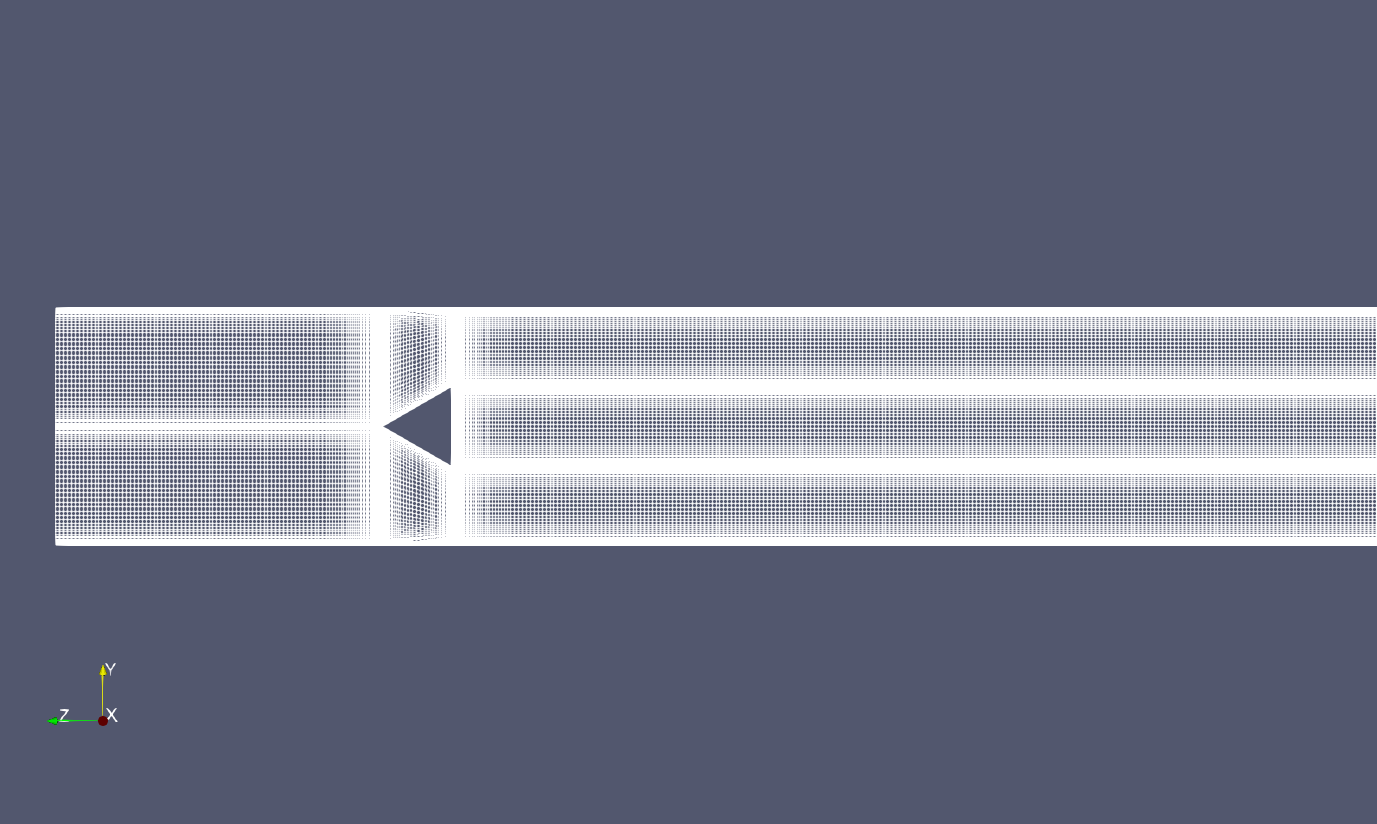
\includegraphics[width=1.2\textwidth]{mesh.png}
   \caption{\SI{2}{\milli\meter} hexagonal mesh, \SI{0.3}{\milli\meter} wall normal distance and clustering near walls; isotropic elsewhere.}
  \end{figure}
  \end{column}
 \end{columns}
 \footnotetext[1]{\fullcite{sjunnesson1991lda}}
 \footnotetext[2]{\fullcite{MVPWorkshop}}
 \footnotetext[3]{\fullcite{COCKS20153394}}
\end{frame}

\begin{frame}
 \frametitle{Non-reacting case}
 Non-reacting simulation velocity profiles validated against experimental results:
 \vskip-2em
 \begin{columns}[t]
  \begin{column}{0.6\textwidth}
   \begin{figure}
    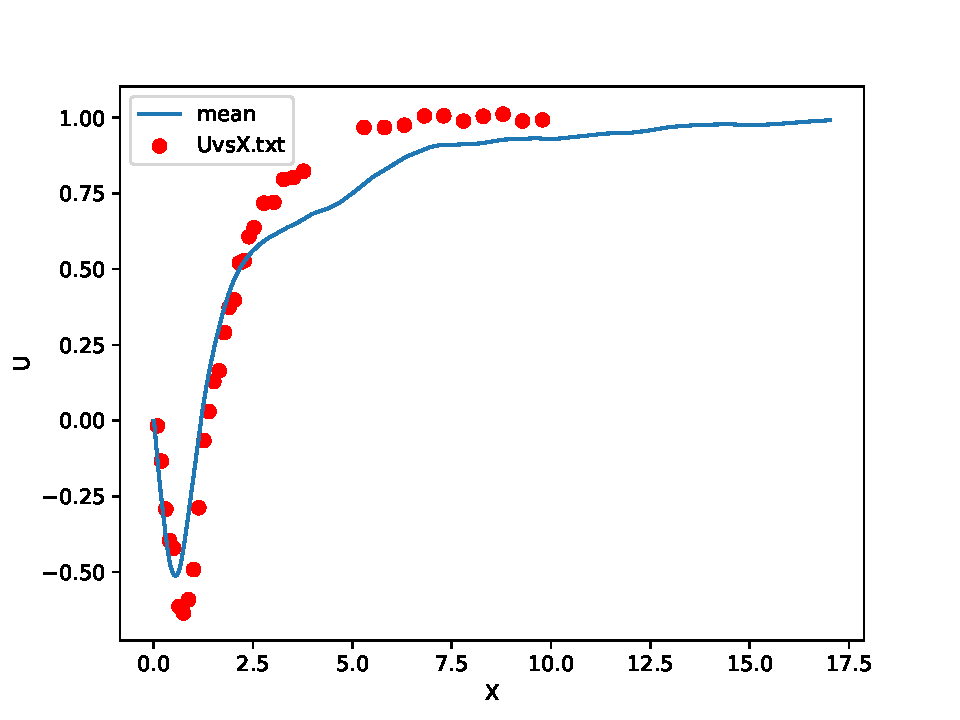
\includegraphics[width=\textwidth]{mean_axial_velocity}
    \caption{Mean-axial velocity comparison.}
   \end{figure}
  \end{column}
  \begin{column}{0.6\textwidth}
  \begin{figure}
   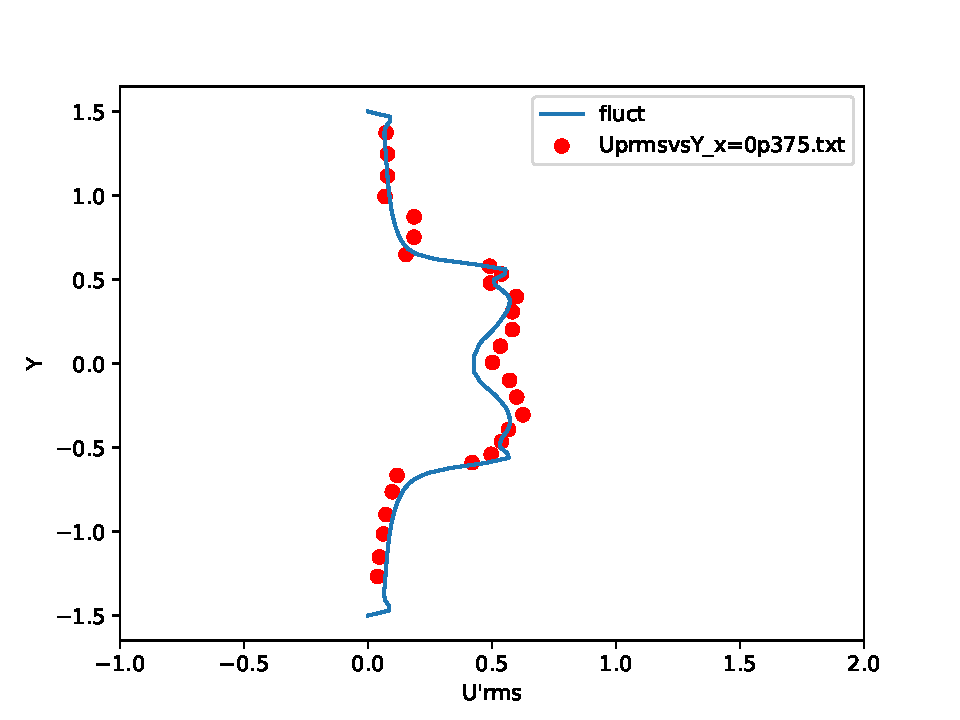
\includegraphics[width=\textwidth]{z_prime_rms_0p375}
   \caption{Axial fluctuation velocity at \num{0.375}D (height of bluff-body) downstream.}
  \end{figure}
  \end{column}
 \end{columns}
\end{frame}

\begin{frame}
 \frametitle{Reacting case}
 In order to obtain a baseline OpenFOAM reacting-flow solution:
 \vskip-1.5em
 \begin{columns}[t]
  \begin{column}{0.6\textwidth}
    \begin{itemize}
      \item Stoichometric methane inflow; ignition kernel positioned behind the bluff body used during flame-development.
      \item Flame ignited using 2-step BFER methane model\note[item]{\fullcite{FRANZELLI2012621}}, switched to GRI-Mech 3.0 once developed.
      \item Fourth-order linearly-implicit Rosenbrock ODE solver\note[item]{faster than either Seulex or Rodas43}, with semi-analytical Jacobian\footnotemark[1]
    \end{itemize}
  \end{column}
  \begin{column}{0.4\textwidth}
   \begin{figure}
    \centering
    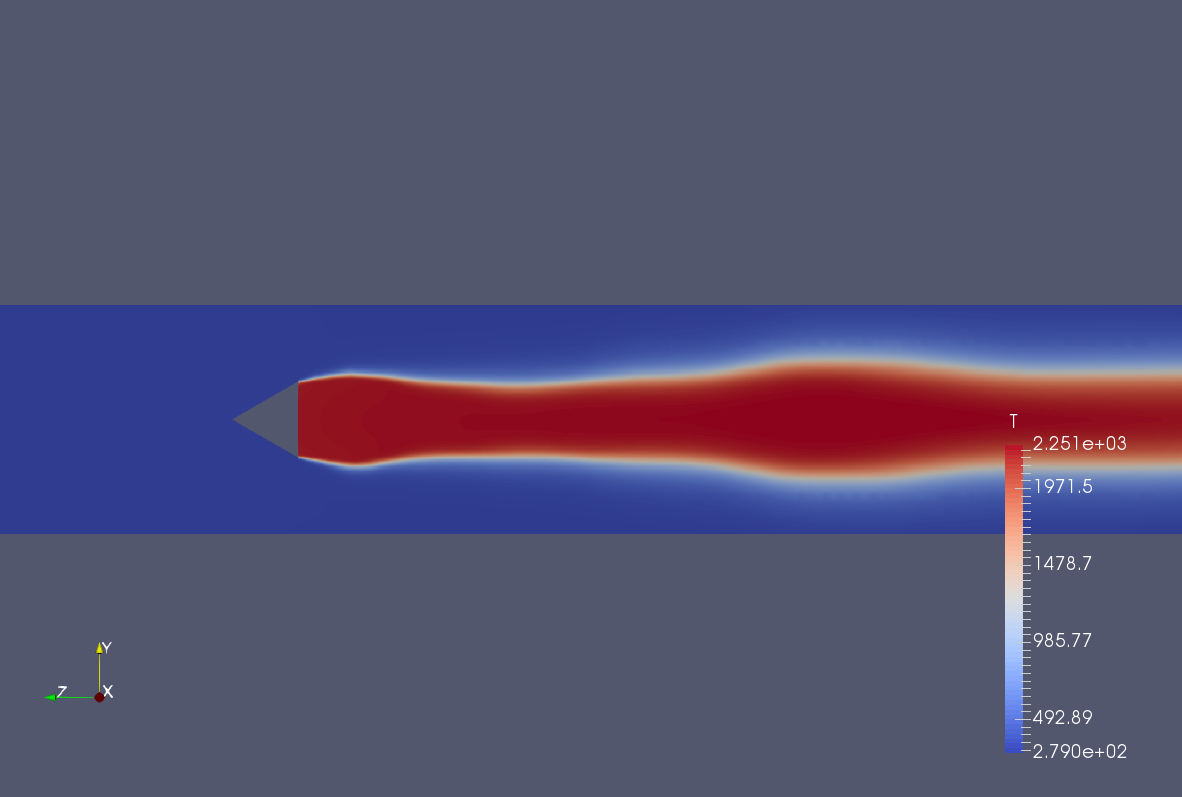
\includegraphics[width=\textwidth]{flame.png}
    \caption{Developed bluff-body stabilized stoichometric methane flame}
   \end{figure}
  \end{column}
 \end{columns}
 \footnotetext[1]{Both are built-in to OpenFOAM}
 Each time-step with the OpenFOAM solvers takes \textapprox\SI{3.5}{\hour} on 92-cores (4-nodes) of UConn HPC.\footnote[2]{In large part due to poor chemistry load-balancing}
 \note[item]{Intel\raisebox{1ex}{\scriptsize{\textregistered}} Xeon\raisebox{1ex}{\scriptsize{\textregistered}} E5-2690 v3 Processor}
\end{frame}

\begin{frame}
 \frametitle{Vectorized solvers}
 As a test of the developed algorithms, we will pair our CPU-vectorized analytical chemical kinetic source term and Jacobian code\footfullcite{CURTIS2018186}, with a previously developed vectorized linearly-implicit Rosenbrock method\footfullcite{STONE201818}, in order to determine:
 \begin{itemize}
  \item Accuracy
  \item Effective speedup
  \item Impact on chemical kinetic integration load-balancing
 \end{itemize}
\end{frame}

\begin{frame}
 \frametitle{Thank you!}
 \large Questions?
\end{frame}


\end{document}